\chapter{Finite automata minimization algorithms}

\section{Introduction}

\section{Brzozowski's algorithm}

\begin{flushleft}
$\epsilon-free$ FA: $M_0=(Q_0,V,T_0,\emptyset,S_0,F_0)$ \\
to be minimized $DFA$: $M_2=(Q_2,V,T_2,\emptyset,S_2,F_2)$ \\
intermediate $NFA$: $M_1=(Q_1,V,T_1,\emptyset,S_1,F_1)$\\
\end{flushleft}

NFA: $M_1 \to $ DFA: $M_2, M_2=suseful_s\circ subsetopt(M_1)$
\begin{align*}
& q_0,q_1\in Q_1,Q_2\subseteq\mathbb{P}(Q_1),\forall p\in  Q_2,p=(q_0,q_1)\\
& \overrightarrow{L}_{M_2}(p)=\overrightarrow{L}_{M_1}(q_0)\cup  \overrightarrow{L}_{M_1}(q_1)\\
& \Rightarrow \\
& \overrightarrow{L}_{M_2}(p)=\bigcup_{q\in p}\overrightarrow{L}_{M_1}(q)\\
& \Rightarrow 
\end{align*}

\begin{figure}[htbp]
	\begin{tikzpicture}
	\matrix (a) [matrix of math nodes,row sep=3em,
	column sep=5em, nodes in empty cells]
	{ Q_1 &  P(Q_1) \\ 
		&  D(Q_2) \\};
	\path[>=latex,->] 
	(a-1-1) edge node [auto] {$subsetopt$} (a-1-2)
	edge node [auto,swap] {$$} (a-2-2)
	(a-1-2) edge node [auto] {$useful_s$} (a-2-2)
	;
	\end{tikzpicture}
	\caption{$M_2=suseful_s\circ subsetopt(M_1)$}
\end{figure}

\begin{figure}[htbp]
	\subfigure[$M_1=(Q_1,V,T_1,\emptyset,S_1,F_1)$] { \label{fig:a} 
	\begin{tikzpicture}[->,>=stealth',shorten >=1pt,auto,node distance=2cm, semithick]
		\tikzstyle{every state}=[minimum size=0.1mm]
		\node[state] (q)  [] {$q$};
		\node[state] (q0) [above right of=q] {$q_0$};
		\node[state] (q1) [below right of=q] {$q_1$};
		\node[state] (f1)  [below right of=q0] {$f_1$};
		\path 
		(q) edge [] node {$a$} (q0)
		    edge [swap] node {$a$} (q1)
		(q0) edge [] node {$\overrightarrow{L}_{M_1}(q_0)$} (f1)
		(q1) edge [swap] node {$\overrightarrow{L}_{M_1}(q_1)$} (f1)
		;
	\end{tikzpicture}
    }
    \hspace{2cm}
	\subfigure[$M_2=(Q_2,V,T_2,\emptyset,S_2,F_2)$] { \label{fig:b}
    \begin{tikzpicture}[->,>=stealth',shorten >=1pt,auto,node distance=3cm, semithick,scale=4]
    	\tikzstyle{every state}=[minimum size=0.1mm]
    	\node[state] (q01)  {$(q_0,q_1)$};
    	\node[state] (f2)  [right of=q01] {$f_2$};
    	\path 
    	(q01) edge [bend left] node {$\overrightarrow{L}_{M_1}(q_0)$} (f2)
    	(q01) edge [bend right,swap] node {$\overrightarrow{L}_{M_1}(q_1)$} (f2)
    	;
    \end{tikzpicture}
    }
	\caption{$M_2=suseful_s\circ subsetopt(M_1)$}
\end{figure}

\begin{figure}[htbp]
	\subfigure[$M_0=(Q_0,V,T_0,\emptyset,S_0,F_0)$] {
		\begin{tikzpicture}[->,>=stealth',shorten >=1pt,auto,node distance=2cm, semithick]
		\tikzstyle{every state}=[minimum size=0.1mm]
		\node[state,accepting] (q2) []{$q_2$};
		\node[state,initial] (q0) [above left of=q2] {$q_0$};
		\node[state] (q1) [above right of=q2] {$q_1$};
		\path
		(q0) edge[bend left] node {$0$} (q1)
		(q1) edge[bend left] node {$0$} (q0)
		(q0) edge[swap] node {$1$} (q2)
		(q1) edge[] node {$1$} (q2)
		(q2) edge[loop below] node {$0,1$} (q2)
		;
		\end{tikzpicture}
	}
    \hspace{1cm}
	\subfigure[$M^R_0=(Q_0,V,T_0,\emptyset,S_0,F_0)^R=(Q_0,V,T^R,\emptyset,F_0,S_0)$]{
		\begin{tikzpicture}[->,>=stealth',shorten >=1pt,auto,node distance=2cm, semithick]
		\tikzstyle{every state}=[minimum size=0.1mm]
		\node[state,initial] (q2) []{$q_2$};
		\node[state,accepting] (q0) [above left of=q2] {$q_0$};
		\node[state] (q1) [above right of=q2] {$q_1$};
		\path
		(q1) edge[bend right,swap] node {$0$} (q0)
		(q0) edge[bend right,swap] node {$0$} (q1)
		(q2) edge[] node {$1$} (q0)
		(q2) edge[swap] node {$1$} (q1)
		(q2) edge[loop below] node {$0,1$} (q2)
		;
		\end{tikzpicture}
	}
    \newline
	\subfigure[$useful_s\circ subsetopt\circ R(M_0)$]{
		\begin{tikzpicture}[->,>=stealth',shorten >=1pt,auto,node distance=2cm, semithick]
		\tikzstyle{every state}=[minimum size=0.1mm]
		\node[state,initial] (q2) []{$q_2$};
		\node[state,accepting] (q0) [above of=q2] {$\{q_0,q_1,q_2\}$};
		\path
		(q2) edge[] node {$1$} (q0)
		(q0) edge[loop above] node {$0,1$} (q0)
		(q2) edge[loop below] node {$0$} (q2)
		;
	\end{tikzpicture}
	}
    \hspace{3cm}
    \subfigure[$M_1=R\circ useful_s\circ subsetopt\circ R(M_0)$]{
    	\begin{tikzpicture}[->,>=stealth',shorten >=1pt,auto,node distance=2cm, semithick]
    	\tikzstyle{every state}=[minimum size=0.1mm]
    	\node[state,accepting] (q2) []{$q_2$};
    	\node[state,initial] (q0) [above of=q2] {$\{q_0,q_1,q_2\}$};
    	\path
    	(q0) edge[] node {$1$} (q2)
    	(q0) edge[loop above] node {$0,1$} (q0)
    	(q2) edge[loop below] node {$0$} (q2)
    	;
    	\end{tikzpicture}
    }
    \caption{$M_1=R\circ useful_s\circ subsetopt\circ R(M_0)$}
\end{figure}

\begin{figure}[htbp]
	\begin{align*}
	\text{start: } &U=\{q_2\}\\
	u=q_2: & T(q_2,0)=\{q_2\},T(q_2,1)=\{q_0,q_1,q_2\} \\
	&\text{add new start to $D$, } D=\{q_2,\{q_0,q_1,q_2\}\} \\
	u=\{q_0,q_1,q_2\}:& T(\{q_0,q_1,q_2\},0)=T(q_0,0)\cup T(q_1,0)\cup T(q_2,0)=\{q_1\}\cup \{q_0\}\cup \{q_2\} =\{q_0,q_1,q_2\}\\
	&T(\{q_0,q_1,q_2\},1)=T(q_0,1)\cup T(q_1,1)\cup T(q_2,1)=\emptyset\cup \emptyset \cup \{q_0,q_1,q_2\}=\{q_0,q_1,q_2\}
	\end{align*}
	
	\subfigure[$M$]{
		\begin{tikzpicture}[->,>=stealth',shorten >=1pt,auto,node distance=2cm, semithick]
		\tikzstyle{every state}=[minimum size=0.1mm]
		\node[state,initial] (q2) []{$q_2$};
		\node[state,accepting] (q0) [above left of=q2] {$q_0$};
		\node[state] (q1) [above right of=q2] {$q_1$};
		\path
		(q1) edge[bend right,swap] node {$0$} (q0)
		(q0) edge[bend right,swap] node {$0$} (q1)
		(q2) edge[] node {$1$} (q0)
		(q2) edge[swap] node {$1$} (q1)
		(q2) edge[loop below] node {$0,1$} (q2)
		;
		\end{tikzpicture}
	}
    \hspace{2cm}
	\subfigure[$useful_s\circ subsetopt(M)$]{
		\begin{tikzpicture}[->,>=stealth',shorten >=1pt,auto,node distance=2cm, semithick]
		\tikzstyle{every state}=[minimum size=0.1mm]
		\node[state,initial] (q2) []{$q_2$};
		\node[state,accepting] (q0) [right of=q2] {$\{q_0,q_1,q_2\}$};
		\path
		(q2) edge[] node {$1$} (q0)
		(q0) edge[loop above] node {$0,1$} (q0)
		(q2) edge[loop above] node {$0$} (q2)
		;
		\end{tikzpicture}
	}
	\caption{$useful_s\circ subsetopt(M)$}
\end{figure}

\section{Minimization by equivalence of states}

\begin{figure}[htbp]
	Equivalence relation $E\subseteq Q\times Q$\\
	$(p,q)\in E\equiv (\overrightarrow{L}(p)=\overrightarrow{L}(q))$\\
	
	\subfigure[$(p,q)\in E$]{
		\begin{tikzpicture}[->,>=stealth',shorten >=1pt,auto,node distance=2cm, semithick]
		\tikzstyle{every state}=[minimum size=0.1mm]
		\node[state,accepting] (f) {$f$};
		\node[state] (p) [above left of=f]{$p$};
		\node[state] (q) [below left of=f]{$q$};
		\path
		(p) edge[] node {$\overrightarrow{L}(p)$} (f)
		(q) edge[swap] node {$\overrightarrow{L}(q)$} (f)
		;
		\end{tikzpicture}
		}
	    \hspace{2cm}
    	\subfigure[$(p,q)\in E$]{
    	\begin{tikzpicture}[->,>=stealth',shorten >=1pt,auto,node distance=2cm, semithick]
    	\tikzstyle{every state}=[minimum size=0.1mm]
    	\node[state,accepting] (f) {$f$};
    	\node[state] (p) [left of=f]{$[p,q]$};
    	\path
    	(p) edge[] node {$\overrightarrow{L}(\#)$} (f)
    	;
    	\end{tikzpicture}
   		}
	\caption{Equivalence relation $E\subseteq Q\times Q$}
\end{figure}

\begin{figure}[htbp]
	$\overrightarrow{L}(p)=\bigcup_{a\in V}(\{a\} \cdot \overrightarrow{L}(T(p,a)) \cup \{\epsilon|p\in F\}$\\

	\begin{tikzpicture}[->,>=stealth',shorten >=1pt,auto,node distance=3cm, semithick]
		\tikzstyle{every state}=[minimum size=0.1mm]
		\node[state,accepting] (p) {$p$};
		\node[state] (q1) [above right of=p]{$T(p,a)$};
		\node[state] (q2) [below right of=p]{$T(p,b)$};
		\node[state,accepting] (f1) [right of=q1]{$f1$};
		\node[state,accepting] (f2) [right of=q2]{$f2$};
		\path
		(p) edge[] node {$a$} (q1)
		(p) edge[] node {$b$} (q2)
		(q1) edge[] node {$\overrightarrow{L}(T(p,a))$} (f1)
		(q2) edge[] node {$\overrightarrow{L}(T(p,b))$} (f2)
		;
	\end{tikzpicture}
	\caption{$L(p)$}
\end{figure}

Let $A=(Q,V,T,_,F)$ be a deterministic finite automaton, where $Q$ is a finite set of states, $V$ is a finite set of input symbols, $T$ is a mapping from $Q\times V$ into $Q$, and $F\subseteq Q$ is the set of final states. No initial state is specified since it is of no importance in what follows. The mapping $T$ is extended to $T\times V^\ast$ in the usual manner where $V^\ast$ denotes the set of all finite strings (including the empty string $\epsilon$) of symbols from $V$

\begin{definition}[equivalent states]
	The states $s$ and $t$ are said to be equivalent if for each $x\in V^\ast, T(s,x)\in F$ if and only if $T(t,x)\in F$. 
\end{definition}

From \cite{Hopcroft71}

The algorithm for finding the equivalence classes of Q is described below:

\begin{algorithm}  
	\caption{The algorithm for finding the equivalence classes of Q}  
	\begin{algorithmic}%[1] %每行显示行号  
		\Require $M=(Q,V,T,_,F)$  
		\Ensure The equivalence classes of $Q$  
		\State Step 1. For each $s\in Q$ and each $a\in V$ construct
		
		$T^{-1}(s,a)=\{t|T(t,a)=s\}$
		
		\State Step 2. construct $B(1)=F, B(2)=Q-F$ and for each $a\in V$ and $1\le i\le 2$ construct
		
		\For{each $a\in V$ }
			\For{$i=1$; $i<n$; $i++$ }  
				\State $\hat{B}(B(i),a)=\{s|s\in B(i) \text{ and } T^{-1}(s,a)\ne \emptyset\}$;
			\EndFor  
		\EndFor 
		\State Step 3. Set $k=3$;
		\State Step 4. For each $a\in V$ construct $L(a)$
		\For{each $a\in V$ }
			\If {$|\hat{B}(B(1),a)| \le |\hat{B}(B(2),a)|$}
				\State $L(a) = \hat{B}(B(1),a)$;
			\Else
	            \State $L(a) = \hat{B}(B(2),a)$; 
			\EndIf
		\EndFor
		\State Step 5. Select $a\in V$ and $i\in L(a)$. The algorithm terminates when $L(a)=\emptyset$ for each $a\in V$.
		\State Step 6. Delete $i$ from $L(a)$.
		\State Step 7. For each $j<k$ such that there exists $t\in B(j)$ with $T(t,a)\in \hat{B}(B(i),a)$, perform steps 7a,7b,7c, and 7d.
		
		\State Step 7a. partition $B(j)$ into
			
			$B^\prime(j)=\{t|T(t,a)\in \hat{B}(B(i),a)\}$ and			
		
			$B^{\prime\prime}(j)=B(j)-B^\prime(j)$
		
		\State Step 7b. Replace $B(j)$ by $B^\prime(j)$ and constant $B(k)=B^{\prime\prime}$. Construct the corresponding $\hat{B}(B(j),a)$ and $\hat{B}(B(k),a)$ for each $a\in V$.
		
		\State Step 7c. For each $a\in V$ modify $L(a)$ as follows.
			\If{$j\notin L(a) \& 0<|\hat{B}(B(j),a)|\le |\hat{B}(B(k)),a|$}
				\State $L(a) = L(a)\cup \{j\}$;
			\Else
				\State $L(a) = L(a)\cup \{k\}$;
			\EndIf 
			
		\State Step 7d. Set $k=k+1$.
		
		\State Step 8. Return to Step 5.
	\end{algorithmic}   
\end{algorithm}

\begin{example}
	$Q=\{1,2,3,4,5,6\},V=\{0,1\},T $ see Fig. \ref{fig:mini-ex1}
	
	The algorithm for finding the equivalence classes of Q is described below: 
	\begin{enumerate}[Step 1. ]
		\item For each $s\in Q$ and each $a\in V$ construct   $T^{-1}(s,a)=\{t|T(t,a)=s\}$\\
			$T^{-1}(1,0)=\emptyset,T^{-1}(2,0)=\{1\},T^{-1}(3,0)=\{2\},\cdots,T^{-1}(6,0)=\{5\}$\\
			$T^{-1}(1,1)=\{1\},T^{-1}(2,1)=\{2\},\cdots T^{-1}(6,1)=\{6\},$
		\item $B(1)=F=\{6\},B(2)=Q-F=\{1,2,3,4,5\}$\\
			for each $a\in V$ and $i\in[1,2]$ construct  $\hat{B}(B(i),a)=\{s|s\in B(i) \text{ and } T^{-1}(s,a)\ne \emptyset\}$;\\
			$\hat{B}(B(1),0)=\{6\},\hat{B}(B(2),0)=\{2,3,4,5\}$ \\
			$\hat{B}(B(1),1)=\{6\},\hat{B}(B(1),1)=\{1,2,3,4,5\}$ \\
		\item Set $k=3$
		\item For each $a\in V$ construct $L(a)$ \\
			$L(0) = \{6\},$ \qquad since $|\hat{B}(B(1),0)|=1\le |\hat{B}(B(2),0)|=4$.\\
			$L(1) = \{6\},$ \qquad since $|\hat{B}(B(1),1)|=1\le |\hat{B}(B(2),1)|=5$.
		\item Select $a\in V$ and $i\in L(a)$. The algorithm terminates when $L(a)=\emptyset$ for each $a\in V$.\\
		    $a=0$\\
		    $i=1,\hat{B}(B(i),0)=\{6\}$
		\item Delete $i$ From $L(a)$.\\
			$L(0)=L(0)-B(i)=\emptyset$
		\item For each $j<k$ such that there exists $t\in B(j)$ with $T(t,a)\in \hat{B}(B(i),a)$, perform steps 7a,7b,7c, and 7d. 
			\begin{enumerate}[Step 7a. ]
				\item Partition $B(j)$ into\\ 
					$B^\prime(j)=\{t|T(t,a)\in \hat{B}(B(i),a)\}=\{5\}$ and\\			
				    $B^{\prime\prime}(j)=B(j)-B^\prime(j)$\\
				\item
			\end{enumerate}
	\end{enumerate}  
\end{example}

\begin{figure}[htbp]
	\begin{tikzpicture}[->,>=stealth',shorten >=1pt,auto,node distance=2cm, semithick]
	\tikzstyle{every state}=[minimum size=0.1mm]
	\node[initial,state] (p1)  {$1$};
	\node[state]         (p2) [right of=p1] {$2$};
	\node[state]         (p3) [right of=p2] {$3$};
	\node[state]         (p4) [right of=p3] {$4$};
	\node[state]         (p5) [right of=p4] {$5$};
	\node[state,accepting] (p6) [right of=p5] {$6$};
	\path
	(p1) edge [loop above] node {1} (p1)
	     edge [] node {0} (p2)
	(p2) edge [loop above] node {1} (p2)
	     edge [] node {0} (p3)
	(p3) edge [loop above] node {1} (p3)
		 edge [] node {0} (p4)
    (p4) edge [loop above] node {1} (p4)
         edge [] node {0} (p5)
    (p5) edge [loop above] node {1} (p5)
         edge [] node {0} (p6)
    (p6) edge [loop above] node {1} (p6)
	;
	\end{tikzpicture}
	\caption{Minimizing example} \label{fig:mini-ex1}
\end{figure}

\begin{example}
	Consider the automaton with $Q=\{a,b,c,d,e\},V={0,1},F=\{d,e\}$, and $T$ is given by the arcs of diagram of Fig. (\ref{fig:mini-ex2}).
	
	\{a,b\} is not equivalent, since $T(a,0)\in F$ but $T(b,0)\notin F$.
	
	\{d,e\} is not equivalent, since $T(d,0)\in F$ but $T(e,0)\notin F$. 
	
	Sets of equivalent states: \{a,c\},\{b\},\{d\},\{e\}
	
	另外一种描述:
	\begin{enumerate}
		\item $(a,b)\notin E$, since $T(a,0)\in F$ but $T(b,0)\notin F$.
		\item $(d,e)\notin E$, since $T(d,0)\in F$ but $T(e,0)\notin F$.
		\item 	$(a,c)\in E$, since	$(a,c)\in E\equiv(a\in F\equiv c\in F)\land (\forall v\in V,(T(a,v),T(c,v)\in E)$ \\
		$(a\notin F,c\notin F)\Rightarrow (a\in F\equiv c\in F)$ \\
		$T(a,0)=T(c,0)=\{d\}\Rightarrow (T(a,0),T(c,0)) \in E$\\
		$T(a,1)=T(c,1)=\{c\}\Rightarrow (T(a,1),T(c,1)) \in E$
	\end{enumerate}

	$\hfill\square$.

	Algorithm:
	\begin{enumerate}
		\item $B_1\leftarrow F; B_2\leftarrow (Q-F)$\\
			  $B_1=\{d,e\}; B_2=\{a,b,c\} $
	    \item $|B_1|=2,|B_2|=3.\Rightarrow L\leftarrow (B_1,c)$ \\
	    $T(d,0) =\{d\}\in F;T(e,0)=\{c\}\notin F$ \\ 
	    $\Rightarrow (d,e)$ is not equivalent states.\\
	    $T(d,1)=\{d\}\in F; T(e,1)=\{e\}\in F. \Rightarrow$ 无法判断。\\
	    $L=(B_1,0);$
	    \item split $(d,c)$ \\
	    $T(d,0)=\{d\}\in F; T(c,0)=\{d\}\notin F$ 无法判断\\
	    $T(d,1)=\{d\}\in F; T(c,1)=\{c\} \notin F$\\
	    $\Rightarrow (d,c)$ is not equivalent states.
	\end{enumerate}
\end{example}

\begin{figure} [htbp]
	\{a,b\},\{d,e\}is not equivalent states. \\
	Sets of equivalent states: \{a,c\},\{b\},\{d\},\{e\}\\
	%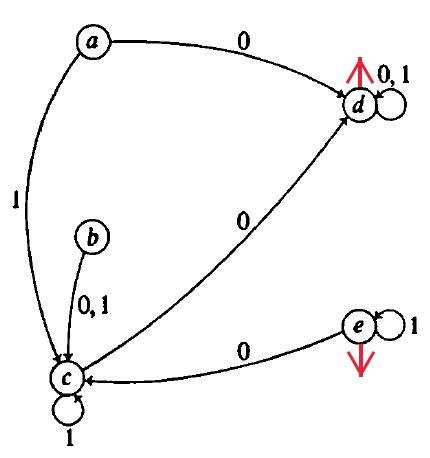
\includegraphics[scale=0.4] {mini-fa} 
	\begin{tikzpicture}[->,>=stealth',shorten >=1pt,auto,node distance=1.5cm, semithick]
	\tikzstyle{every state}=[minimum size=0.1mm]
	\node[state] (a) {$a$};
	\node[state,accepting] (d) [right of=a] {$d$};
	\node[state] (c) [below of=a] {$c$};
	\node[state] (b) [left of=c] {$b$};
	\node[state,accepting] (e) [right of=c] {$e$};
	\path
	(d) edge [loop above] node {$0,1$} (d)
	(c) edge [loop below] node {$1$} (c)
	(e) edge [loop below] node {$1$} (e)
	(a) edge [] node {$0$} (d)
	(a) edge [swap] node {$1$} (c)
	(b) edge [swap] node {$0,1$} (c)
	(e) edge [] node {$0$} (c)
	(c) edge [] node {$0$} (d)
	;
	\end{tikzpicture}
	\caption{Finite state automaton}
	\label{fig:mini-ex2}
\end{figure}

%%%%%%%%%%%%%%%%%%%%%%%%%%%%%%%%%%%%%%%%%%%%%%%%%%5
\begin{thebibliography}{99}
	\bibitem[Hopcroft71]{Hopcroft71}
	Hopcroft, J.E. \textit{An n log n algorithm for minimizing states in a finite automaton}, in The Theory of Machines and Computations (Z. Kohavi, ed.), pp.180-196, Academic Press, New York, 1971.
	
	\bibitem[Gries73]{Gries73}
	Gries, D. \textit{Describing an Algorith m by Hopcroft}, Acta Inf. 2:97 109, 173. $\copyright$ by Springer-Verlag 1973
\end{thebibliography}
